% Created 2024-03-22 Fri 16:00
% Intended LaTeX compiler: pdflatex
\documentclass[11pt]{article}
\usepackage[utf8]{inputenc}
\usepackage[T1]{fontenc}
\usepackage{graphicx}
\usepackage{longtable}
\usepackage{wrapfig}
\usepackage{rotating}
\usepackage[normalem]{ulem}
\usepackage{amsmath}
\usepackage{amssymb}
\usepackage{capt-of}
\usepackage{hyperref}
\bibliographystyle{ieeetr}
\date{\today}
\title{RIMANUS Meeting 20240322}
\hypersetup{
 pdfauthor={},
 pdftitle={RIMANUS Meeting 20240322},
 pdfkeywords={},
 pdfsubject={},
 pdfcreator={Emacs 29.2 (Org mode 9.6.15)}, 
 pdflang={English}}
\begin{document}

\maketitle

\section{Scenario: Unprotected Loss of Flow (ULOF) in SFR (Almost impossible)}
\label{sec:org555f727}
\begin{itemize}
\item Complete failure of redundant shutdown systems (Suzuki, Tohru and Tobita, Yoshiharu and Kawada, Kenichi and Tagami, Hirotaka and Sogabe, Joji and Matsuba, Kenichi and Ito, Kei and Ohshima, Hiroyuki, 2015)
\item Failure forced circulation (e.g. Station Blackout) (Zhao, Haiqi and Lu, Daogang and Zhang, Yuhao and Zhang, Xueyuan, 2023)
\item Thermal mixing happens primarily due to natural convection (Guenadou, David, 2022)
\end{itemize}
\cite{ZusatzversorgungOeffentlichenDienstes}
\bibliography{mylib/bib/mylib}
\cite{zuoTwodimensionalNumericalSimulation2013}
\section{What is the natural circulation/convection?}
\label{sec:org9011da3}
\begin{itemize}
\item Sodium: high thermal conductivity (Ishida, Shinya and Kawada, Ken-ichi and Fukano, Yoshitaka, 2020)
\item Thermal stratification in sodium pool (Zhao, Haiqi and Lu, Daogang and Zhang, Yuhao and Zhang, Xueyuan, 2023)
\item Induced by temperature difference of coolant at the inlet and outlet of the core (, 2015)
\item Temperature difference --> Density difference --> Convection (Guenadou, David, 2022)
\item Decay heat removed without electricity (, 2015)
\item One of the most important mechanisms of passive safety (, 2015)
\end{itemize}

\section{How fast is the natural convection? (Guenadou, David, 2022)(Zhao, Haiqi and Lu, Daogang and Zhang, Yuhao and Zhang, Xueyuan, 2023)}
\label{sec:org591c077}
\begin{itemize}
\item Locally different
\item No more than 0.6m/s
\item Lack of study until 2022 (Guenadou, David, 2022)
\end{itemize}

\section{From natural circulation to \href{20240307154931-core_disruptive_accident_cda.org}{Core Disruptive Accident (CDA)}}
\label{sec:orgd855605}
\begin{itemize}
\item 15 hours from failure of forced circulation to total sodium boiling without natural circulation (Bachrata, Andrea and Bertrand, Fr{\'e}deric and Marie, Nathalie and Serre, Fr{\'e}deric, 2021)
\end{itemize}

\section{What is the process of CDA? (Ishida, Shinya and Kawada, Ken-ichi and Fukano, Yoshitaka, 2020)}
\label{sec:org1d0c949}
\begin{itemize}
\item Initial Phase (IP)
\item Transition Phase (TP)
\item Post-Accident Material Relocation/Post-Accident Heat Removal (PAMR/PAHR) phase
\item \href{images/CDA.png}{Sketch of CDA}
\begin{center}
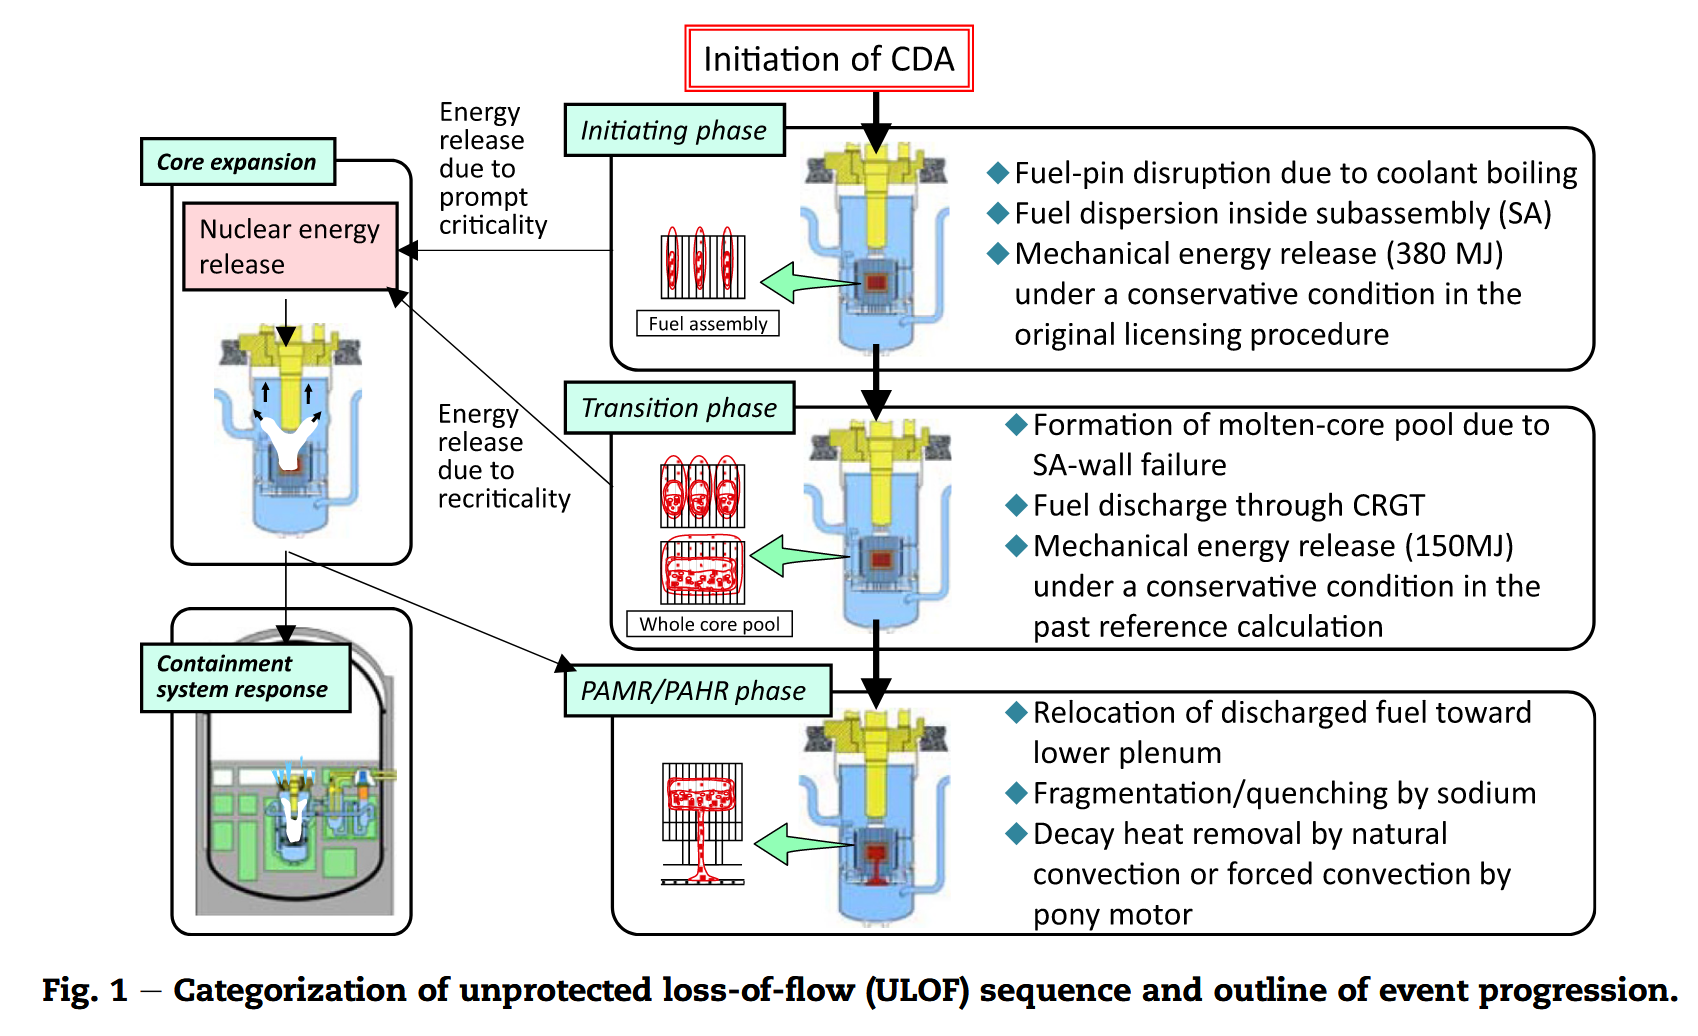
\includegraphics[width=.9\linewidth]{images/CDA.png}
\end{center}
\item \href{images/framework\_code.png}{Components of the meltdown}
\begin{center}
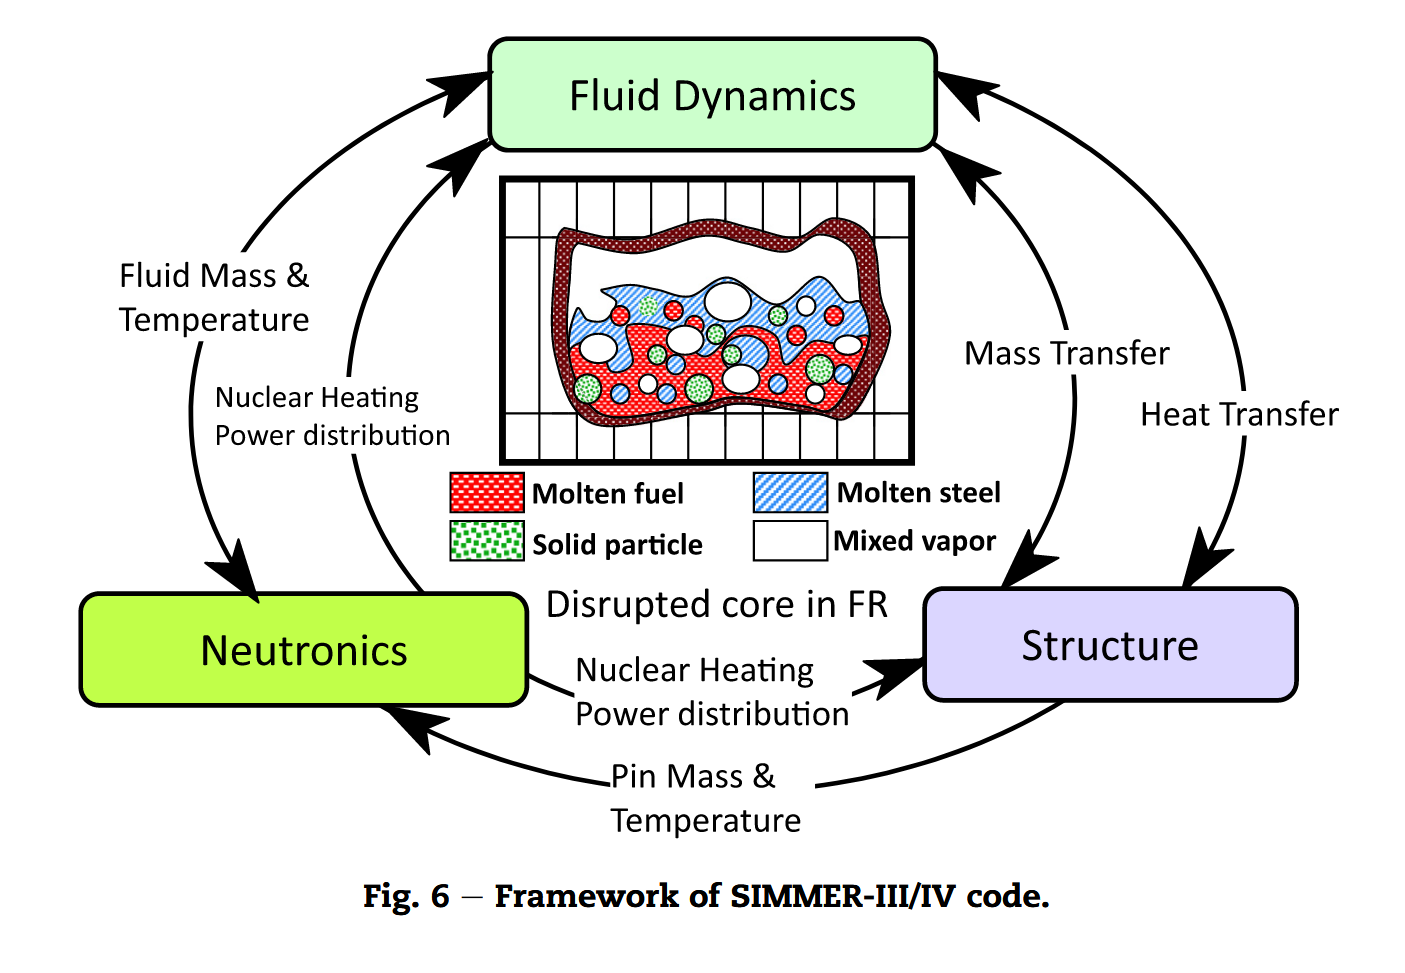
\includegraphics[width=.9\linewidth]{images/framework_code.png}
\end{center}
\item \href{images/transient.png}{Transient of reactivity and power in initiating phase}
\begin{center}
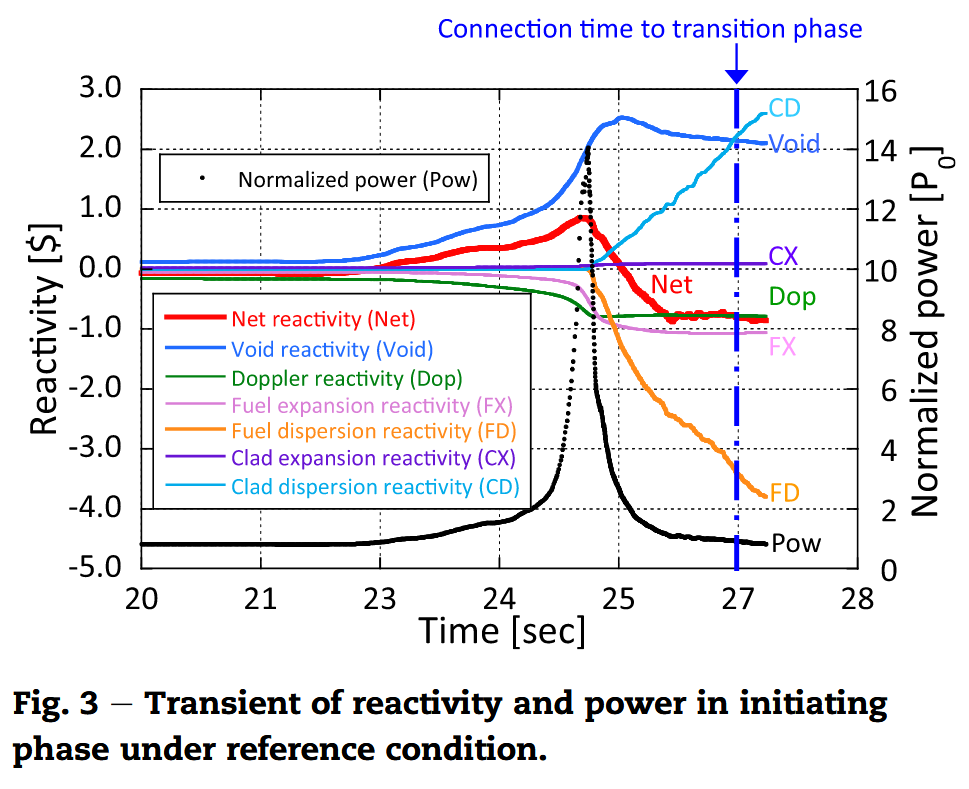
\includegraphics[width=.9\linewidth]{images/transient.png}
\end{center}
\item \href{images/components.png}{Components of the mixture}
\begin{center}
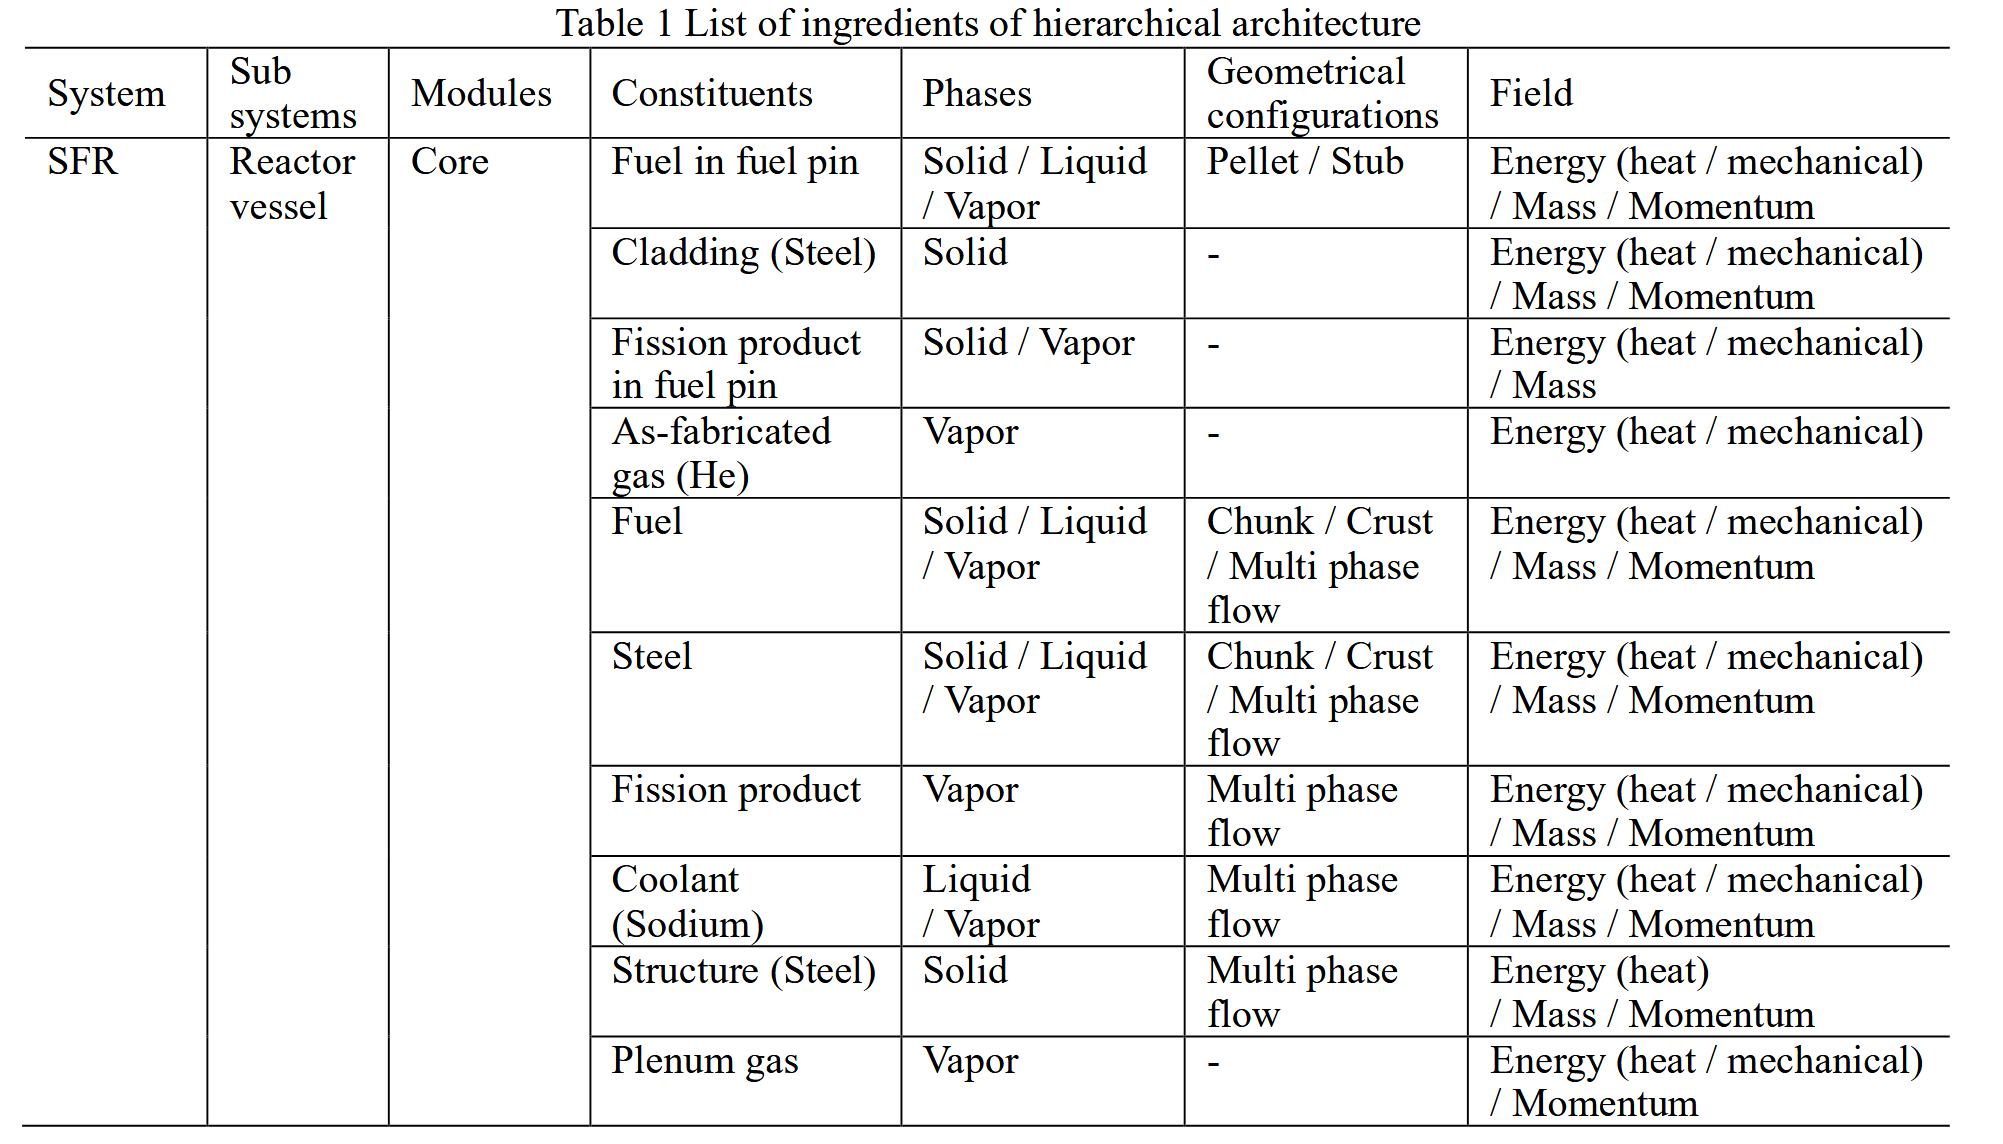
\includegraphics[width=.9\linewidth]{images/components.png}
\end{center}
\end{itemize}

\section{About viscosity}
\label{sec:orgfe32178}
\begin{itemize}
\item \href{20240313140039-viscosity.org}{Viscosity} \(\uparrow\) Coalescence \(\downarrow\) (Important)
\end{itemize}

\section{Quotes}
\label{sec:org231f729}
\begin{quote}
The reduction of the coolant flow causes (1) the fuel temperature rise and (2) the fuel thermal expansion, and the thermal expansion changes the fuel-cladding gap width. This change affects (3) the gap conductance and the thermal condition changes accordingly. The events progress while the thermal behavior and the mechanical behavior interact with each other. The coolant gradually boils and it causes the cladding temperature rise. In an assembly where the strength of the cladding is sufficiently degraded due to the temperature rise, (4) the fuel pellets temperature rises, the molten cavities develop, and (5) the fuel is disrupted when the fuel pellets cannot maintain their shape due to the strength degradation. Hence, the fuel disruption largely depends on the fuel pin thermal behavior and the fuel pin mechanical behavior. Furthermore, when the power excursion occurs due to the positive reactivity insertion which is caused by the coolant boiling, (6) the pressure applied by the fuel to the cladding, which is called the contact pressure, causes (7) the fuel pin failure in an assembly where the cladding keeps the strength due to sufficient cooling. (Ishida, Shinya and Kawada, Ken-ichi and Fukano, Yoshitaka, 2020)
\end{quote}
\begin{quote}
Experiments show that the viscosity has a greater impact on the bubble coalescence. The greater the viscosity, the harder the bubbles are to coalesce. (Dai, Caili and Zhao, Guang and You, Qing and Zhao, Mingwei and Liu, Yifei and Zhao, Fulin, 2022)
\end{quote}
\cite{afflardBubbleDetectionLiquid2023}
\section{Bibliography}
\label{sec:org9104dee}
\noindent
Bachrata, Andrea and Bertrand, Fr{\'e}deric and Marie, Nathalie and Serre, Fr{\'e}deric (2021). \emph{A Comparative Study on Severe Accident Phenomena Related to Melt Progression in {{SFR}} and {{PWR}}}, ASME.

\noindent
Dai, Caili and Zhao, Guang and You, Qing and Zhao, Mingwei and Liu, Yifei and Zhao, Fulin (2022). \emph{Theory and Technology of Multiscale Dispersed Particle Gel for In-Depth Profile Control}, Elsevier.

\noindent
Guenadou, David (2022). \emph{107 {{PUBLICATIONS}} 780 {{CITATIONS SEE PROFILE}}}.

\noindent
Ishida, Shinya and Kawada, Ken-ichi and Fukano, Yoshitaka (2020). \emph{Validation Study of {{SAS4A}} Code for the Unprotected Loss-of-Flow Accident in an {{SFR}}}, Mechanical Engineering Journal.

\noindent
 (2015). \emph{Analysis of {{Natural Circulation Tests}} in the {{Experimental Fast Reactor JOYO}}}.

\noindent
Suzuki, Tohru and Tobita, Yoshiharu and Kawada, Kenichi and Tagami, Hirotaka and Sogabe, Joji and Matsuba, Kenichi and Ito, Kei and Ohshima, Hiroyuki (2015). \emph{A Preliminary Evaluation of Unprotected Loss-of-Flow Accident for a Prototype Fast-Breeder Reactor}, Nuclear Engineering and Technology.

\noindent
Zhao, Haiqi and Lu, Daogang and Zhang, Yuhao and Zhang, Xueyuan (2023). \emph{Numerical Simulation of Natural Circulation Characteristics under Different {{DHX}} Layout Schemes in Pool-Type {{SFR}} during Station Blackout Accident}, Progress in Nuclear Energy.
\bibliographystyle{plain}
\bibliography{mylib/bib/mylib}
\end{document}
